\subsection{Analytical Comparisons}

This section compares the simulated results with the analytical solution of ACE. I begin with the consumption rate and the abatement rate, continue with the costate variables and the SCC they imply, and end with the simulated paths of the states. Throughout, the figures show the paths up to the year 2300, and the policy network is evaluated along its own simulated trajectory. Table (\ref{table:comparison}) summarizes the main comparisons.

\begin{table}[ht]
\centering
\begin{adjustbox}{width=\textwidth,center}
\begin{tabular}{lcccc}
\toprule
 & \multicolumn{2}{c}{ACE-DICE 2016} & \multicolumn{2}{c}{ACE-DICE 2023} \\
\cmidrule(lr){2-3} \cmidrule(lr){4-5}
 & DEQN & Analytic & DEQN & Analytic \\
\midrule
Consumption rate $x$ (mean to 2300) & 0.7394 & 0.7395 & 0.7396 & 0.7395 \\
Costate $\lambda_k$ & 0.3524 & 0.3524 & 0.3520 & 0.3524 \\
Costate $\lambda_{M_1}$ ($\times 10^{-4}$) & -1.046 & -1.046 & -1.044 & -1.046 \\
Costate $\lambda_{\tau_1}$ & -0.0559 & -0.0559 & -0.0559 & -0.0559 \\
SCC in 2050 (USD/tCO$_2$) & 36.9 & 37.0 & 37.3 & 37.4 \\
Temperature in 2100 (°C) & 2.96 & 2.96 & 3.47 & 3.47 \\
Peak temperature (°C) & 3.33 & 3.33 & 4.71 & 4.72 \\
\midrule
Abatement rate, mean $|\mu - \mu^*|$ & \multicolumn{2}{c}{0.0009} & \multicolumn{2}{c}{0.0020} \\
Abatement rate, max $|\mu - \mu^*|$ & \multicolumn{2}{c}{0.0166} & \multicolumn{2}{c}{0.0227} \\
\bottomrule
\end{tabular}

\end{adjustbox}
\caption{Policy network (DEQN) against the analytical solution. Costates are averaged over the periods up to 2300; the abatement rate errors are taken over the same periods.}
\label{table:comparison}
\end{table}

\subsubsection{The Consumption Rate}

As shown in equation (\ref{eq:analytical_x_t}), the optimal consumption rate is constant over time and independent of the states visited, \(x^* = 1 - \beta\kappa \approx 0.7395\). The upper panels of Figure (\ref{fig:controls}) show the consumption rates estimated by the policy network, together with the analytical rate and the consumption rates estimated with the original implementation.

\begin{figure}[ht]
  \centering
  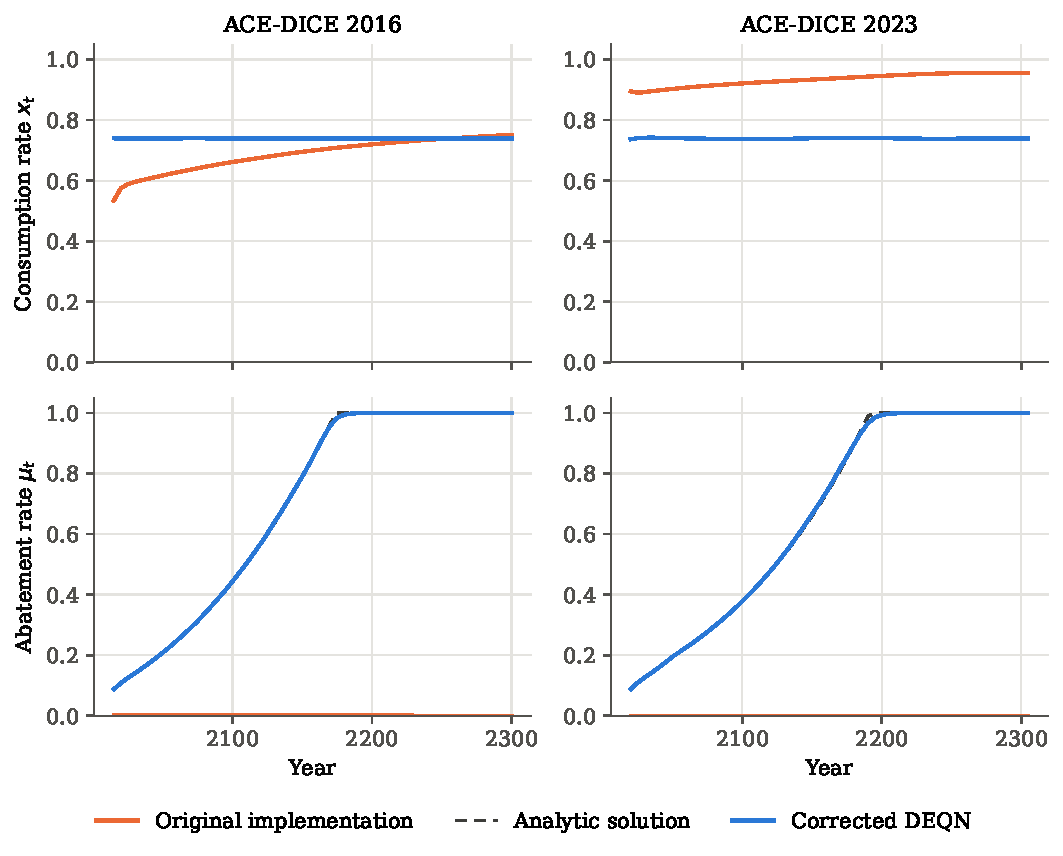
\includegraphics[width=1.0\textwidth]{images/ch6/revised/controls.pdf}
  \caption{Consumption rate (top) and abatement rate (bottom): corrected DEQN, analytical solution and original implementation}
  \label{fig:controls}
\end{figure}

The estimated consumption rates match the analytical solution closely. Over the periods up to 2300, the largest deviation from \(x^*\) is \(6 \cdot 10^{-4}\) for the 2016 version and \(2.8 \cdot 10^{-3}\) for the 2023 version, and the policy network has learned that the consumption rate does not depend on the state. In contrast, the original implementation estimated a consumption rate that rises from about 0.53 to 0.75 for the 2016 version and lies above 0.89 for the 2023 version. These deviations were not caused by the normalization of inputs, as suggested in the submitted version of this thesis, but by the errors in the capital condition \(\ell_0\) and the consumption condition \(\ell_3\): at the analytical solution, the original conditions are not zero, so the network was trained towards a different fixed point.

\subsubsection{The Abatement Rate}

Given the carbon price implied by the costate variables, the optimal abatement rate solves the first-order condition on emissions (eq. \ref{eq:general_objective_4}), which is equivalent to equation (\ref{eq:analytical_abatement_rate}) with \(\Gamma_t = SCC_t\). Where the solution exceeds one, the constraint \(E_t \geq 0\) binds and the abatement rate is one.

The lower panels of Figure (\ref{fig:controls}) show that the estimated abatement rates follow the analytical rates closely, from about 9\% in the first period to full abatement in 2175 for the 2016 version and in 2195 for the 2023 version. The mean absolute deviation over the periods up to 2300 is 0.0009 for the 2016 version and 0.0020 for the 2023 version. The largest deviations, of about 0.02, occur in the few periods around the kink where the abatement rate reaches one, which the smooth policy network rounds off. The original implementation estimated abatement rates close to zero in both versions.

\subsubsection{Costate Variables and the Social Cost of Carbon}

The costate variables of ACE are constant along the optimal path (Appendix \ref{appendix:supplementary_figures}). The policy network recovers them with a largest relative deviation over the periods up to 2300 of 0.3\% for \(\lambda_k\), 0.5\% for \(\lambda_{M_1}\) and 0.4\% for \(\lambda_{\tau_1}\) in the 2016 version, and of 1.4\%, 1.4\% and 0.5\% in the 2023 version. This is notable for the carbon costate \(\lambda_{M_1} \approx -1.05 \cdot 10^{-4}\), which is four orders of magnitude smaller than \(\lambda_k\) and is only identified through the conditions on the carbon cycle and on emissions. Without the scaling of section (\ref{subsubsec:objective_scaling}), these conditions carry almost no weight in the policy objective.

\begin{figure}[ht]
  \centering
  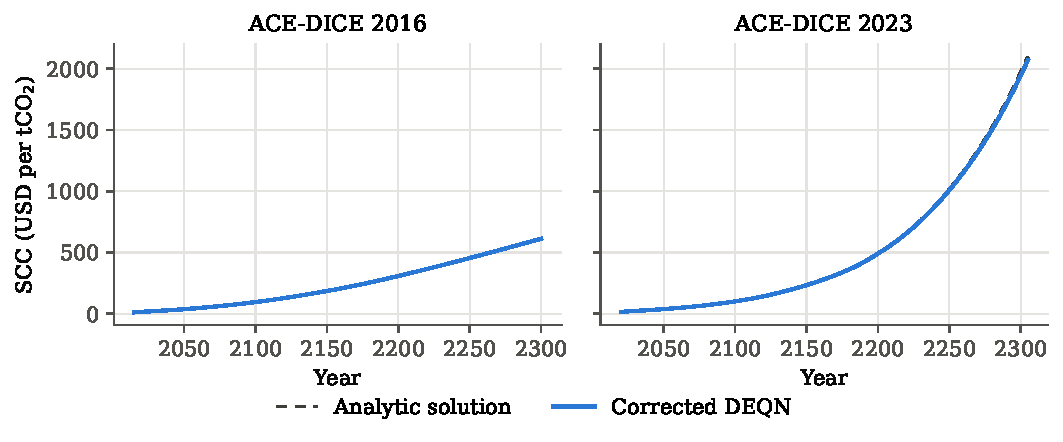
\includegraphics[width=1.0\textwidth]{images/ch6/revised/scc.pdf}
  \caption{SCC in USD/tCO$_2$ implied by the policy network and the analytical solution}
  \label{fig:social_cost_of_carbon_plot}
\end{figure}

Figure (\ref{fig:social_cost_of_carbon_plot}) shows the SCC implied by the costates of the policy network, as given below equation (\ref{eq:analytical_scc}), together with the analytical SCC (eq. \ref{eq:analytical_scc}) evaluated at the same states. The two are almost indistinguishable. For the 2016 version, the SCC rises from 11.1 USD/tCO\(_2\) in 2015 (analytical: 11.0) to 95.1 USD/tCO\(_2\) in 2100 (95.1). For the 2023 version, it rises from 14.1 USD/tCO\(_2\) in 2020 (14.2) to 100.5 USD/tCO\(_2\) in 2100 (100.9). The SCC is proportional to net output, so it grows faster in the 2023 version, where total factor productivity grows faster.

\subsubsection{Simulated Paths}

Figure (\ref{fig:states}) compares the states along the trajectory simulated with the policy network to the optimal path obtained by simulating the analytical controls from the same initial state. Since the estimated controls are close to optimal, the two paths coincide. In the 2016 version, atmospheric temperature peaks at 3.33°C around 2150 and atmospheric carbon at about 1590 GtC. In the 2023 version, where emissions are higher because of faster output growth, temperature peaks at 4.71°C around 2185 (analytical: 4.72°C). The small differences after 2200 in the 2023 version reflect the deviations in the abatement rate around the kink.

\begin{figure}[ht]
  \centering
  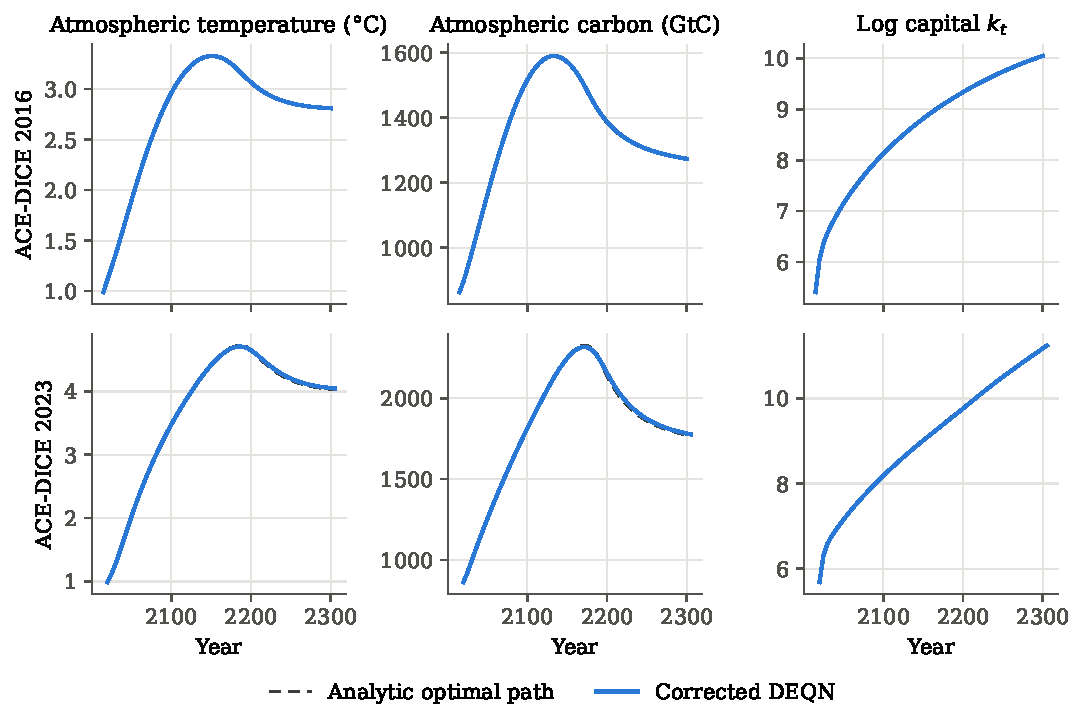
\includegraphics[width=1.0\textwidth]{images/ch6/revised/states.pdf}
  \caption{Atmospheric temperature, atmospheric carbon and log capital along the trajectory simulated with the policy network and along the analytical optimal path}
  \label{fig:states}
\end{figure}
